%%%%%%%%%%%%%%%%%%%%%%%%%%%%%%%%%%%%%%%%%%%%%%%%%%%%%%%%%%
%% BEGIN PREAMBLE
\documentclass[10pt]{article}

%%%% Sets 1 inch margins on document
\usepackage[margin=1in]{geometry}

%%%% For math macros
\usepackage{amsmath}

%%%% Needed for including figures and other images
\usepackage{graphicx}

%%%% Adds ability to adjust document vertical spacing
% usage:
%   \setspace{1.5} % 1.5x for line spacing
\usepackage{setspace}

%%%% Needed for specifying the list items in enumerate env
% eg. (a,b,b) or (i,ii,iii), (1,2,3)
% usage:
%   \begin{enumerate} [label=(\alph*)] % for (a), (b), (c)
\usepackage{enumitem}

%%%% Defines Times New Roman as font
  % for math and text environments
\usepackage{newtxtext,newtxmath}

%%%% For H float option when inserting figure
%   [H] inserts figure _exactly_ where it is typeset
% usage:
%   begin{figure} [H]
\usepackage{float}

%%%% For fancy header and footer ;)
\usepackage{fancyhdr}
\pagestyle{fancy}
\fancyhead[LO,L]{Samuel Barton}
\fancyhead[CO,C]{ENGS31 - Homework 1}
\fancyhead[RO,R]{\today}
\fancyfoot[LO,L]{}
\fancyfoot[CO,C]{\thepage}
\fancyfoot[RO,R]{}
\renewcommand{\headrulewidth}{0.4pt}
\renewcommand{\footrulewidth}{0.4pt}

%%%% Setting margins in tabular environments
% For making equations (esp. fractions) fit in cells vertically
\usepackage{cellspace}
\cellspacetoplimit 4pt
\cellspacebottomlimit 4pt
%% END PREAMBLE %%
%%%%%%%%%%%%%%%%%%%%%%%%%%%%%%%%%%%%%%%%%%%%%%%%%%%%%%%%%%%%%%%

\begin{document}

\setstretch{1.25} % set spacing to 1.25x

% Assignment Name
\begin{centering}
  \section*{HOMEWORK 1}
\end{centering}

\begin{enumerate}
  \item
  \begin{enumerate}
    \item 
      BIN: \texttt{10101101} \\
      HEX: \texttt{0xAD} \\
      BCD: \texttt{0001 0111 0011}
    \item 
      BIN: \texttt{0111111} \\
      HEX: \texttt{0x7F} \\
      BCD: \texttt{0001 0010 0111}
    \item 
      BIN: \texttt{01010100} \\
      HEX: \texttt{0x54} \\
      BCD: \texttt{0110 1000}
  \end{enumerate}
  \item 
  \begin{enumerate}
    \item 
      HEX: \texttt{0x69} \\
      DEC: 105 \\
      BCD: 69
    \item 
      HEX: \texttt{0x48} \\
      DEC: 72 \\
      BCD: 48
    \item 
      HEX: \texttt{0x5E} \\
      DEC: 94
      BCD: N/A
  \end{enumerate}
  \item 
  \begin{enumerate}
    \item 
      \begin{gather*}
        A=W'X'Y'+W'X'Y+W'XY'+WX'Y'+WX'Y+WXY' \\
        B=W'X'Y+W'XY+WX'Y+WXY' \\
        C=W'XY'+W'XY+WX'Y'+WX'Y
      \end{gather*}
      \begin{figure} [H]
      \begin{tabular}{c}
        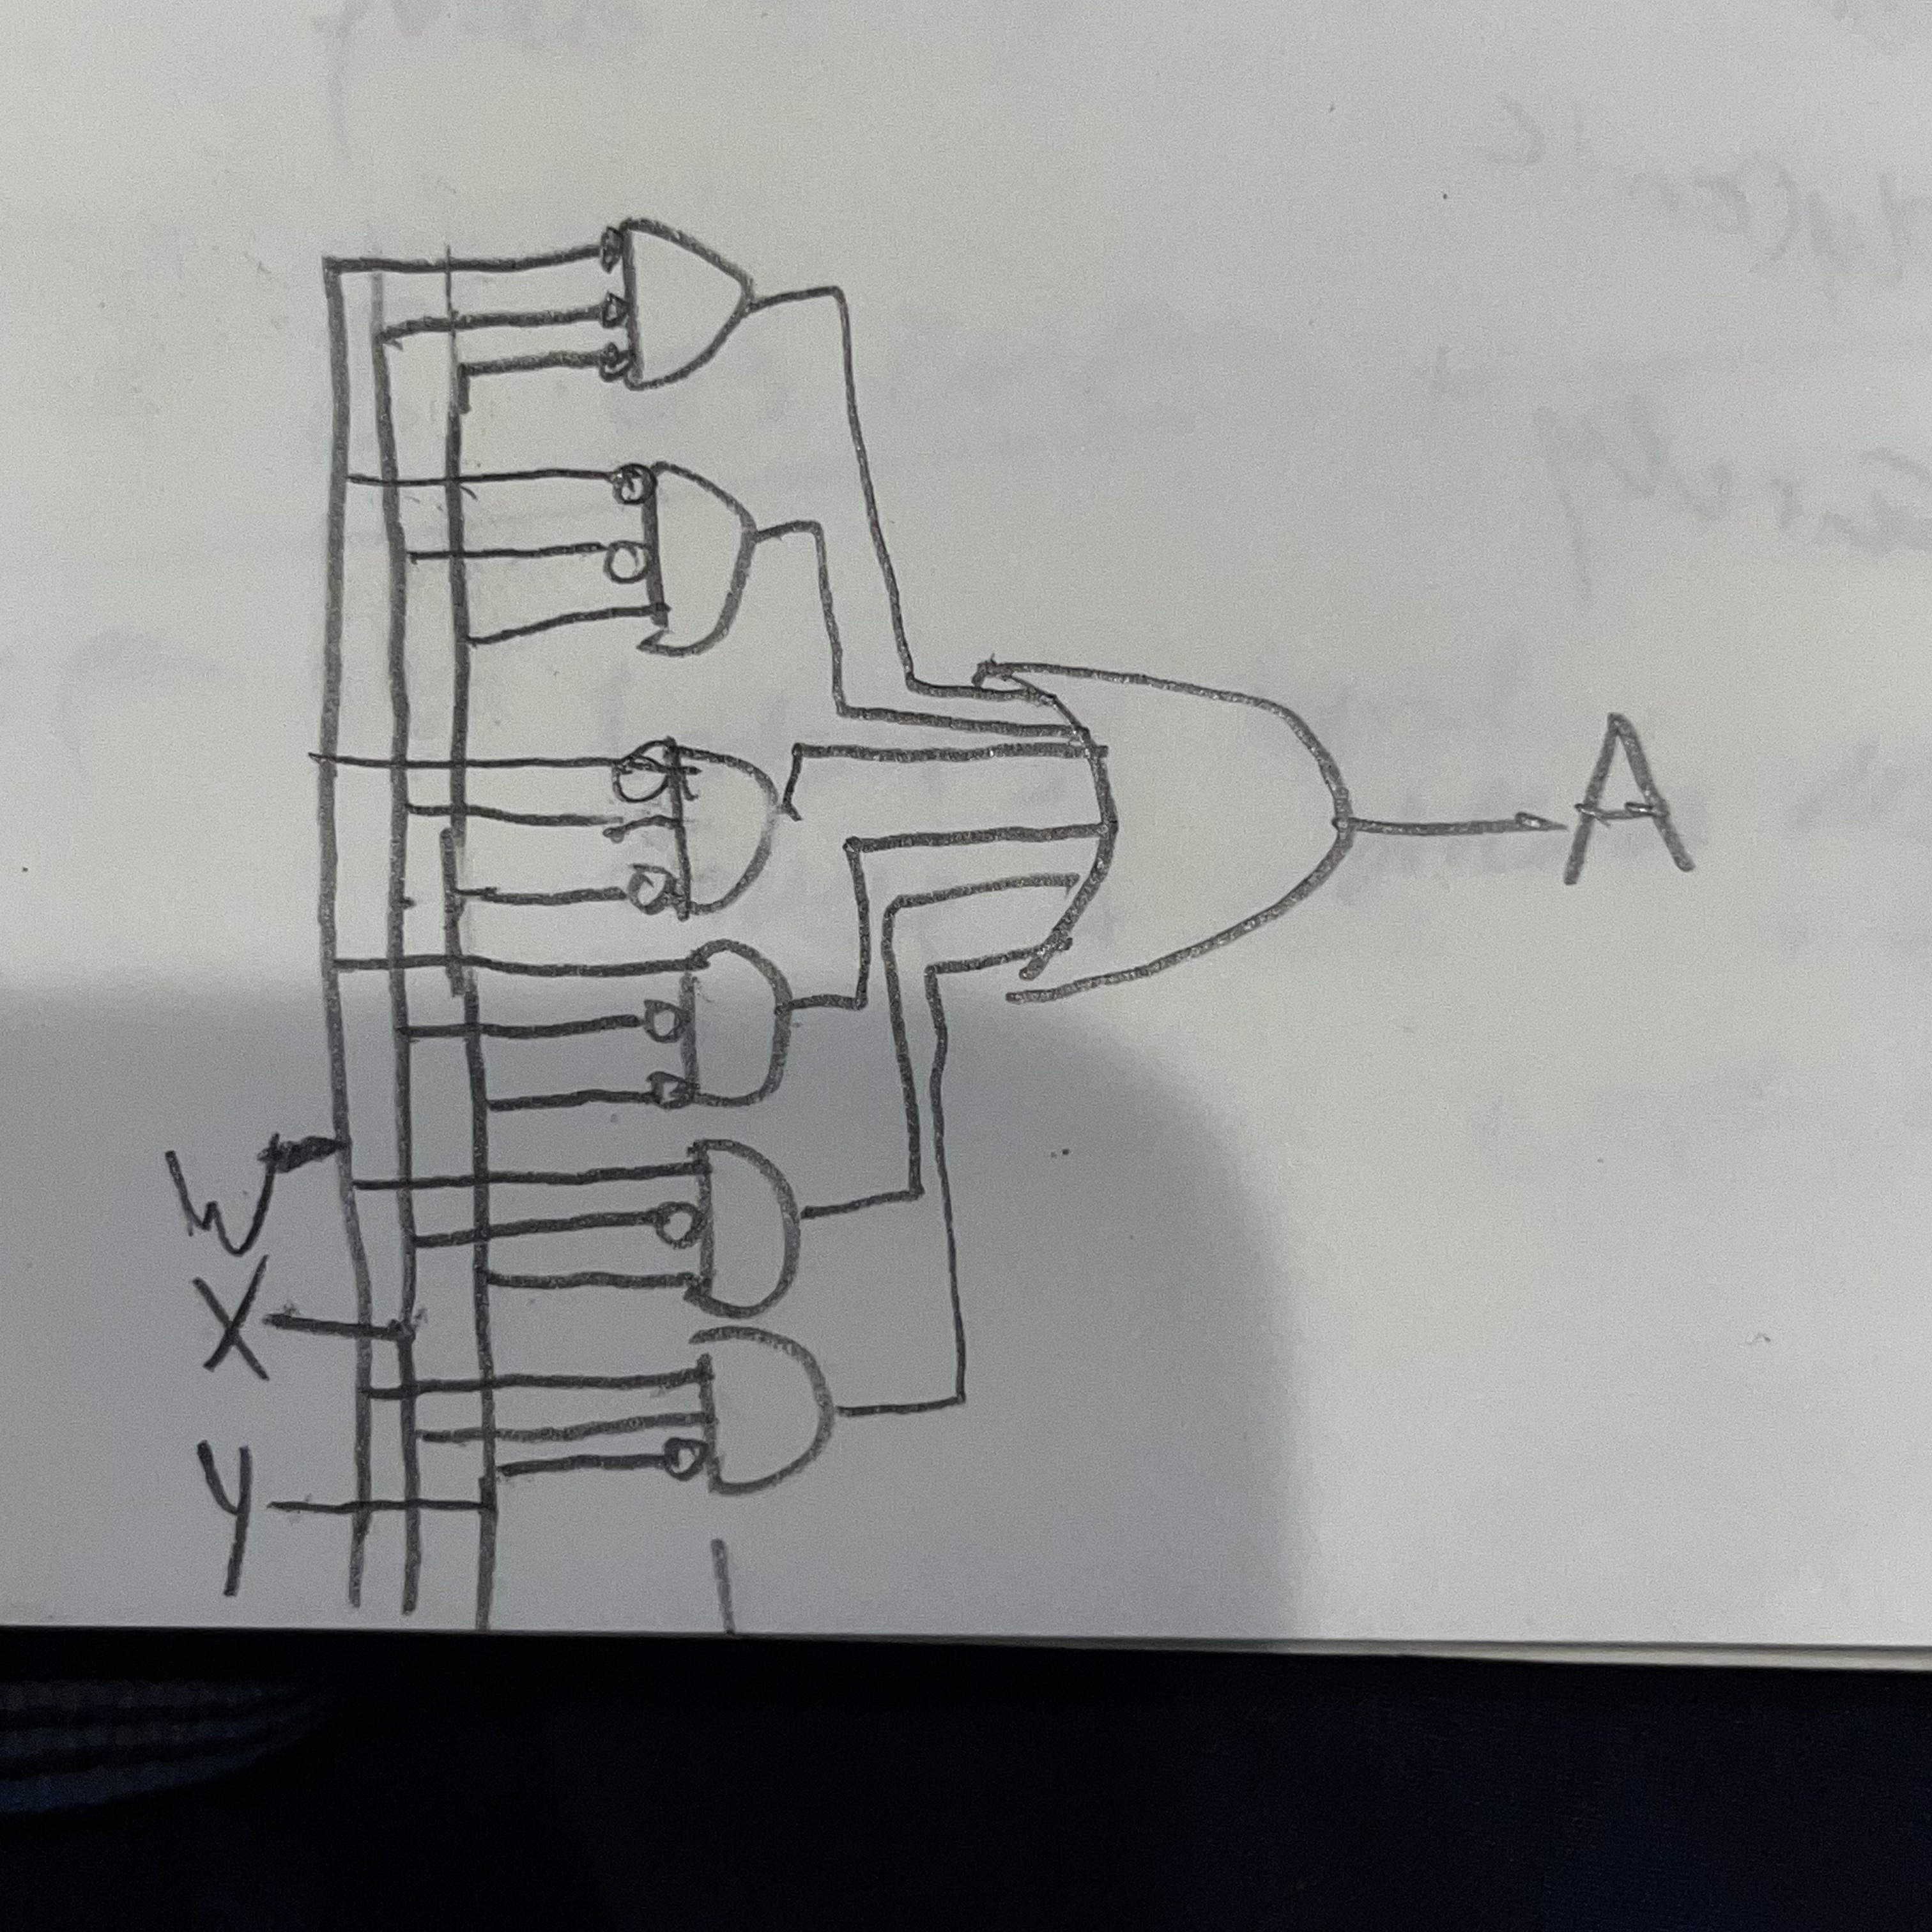
\includegraphics[width=0.3\textwidth]{./Images/A.jpeg}\\
        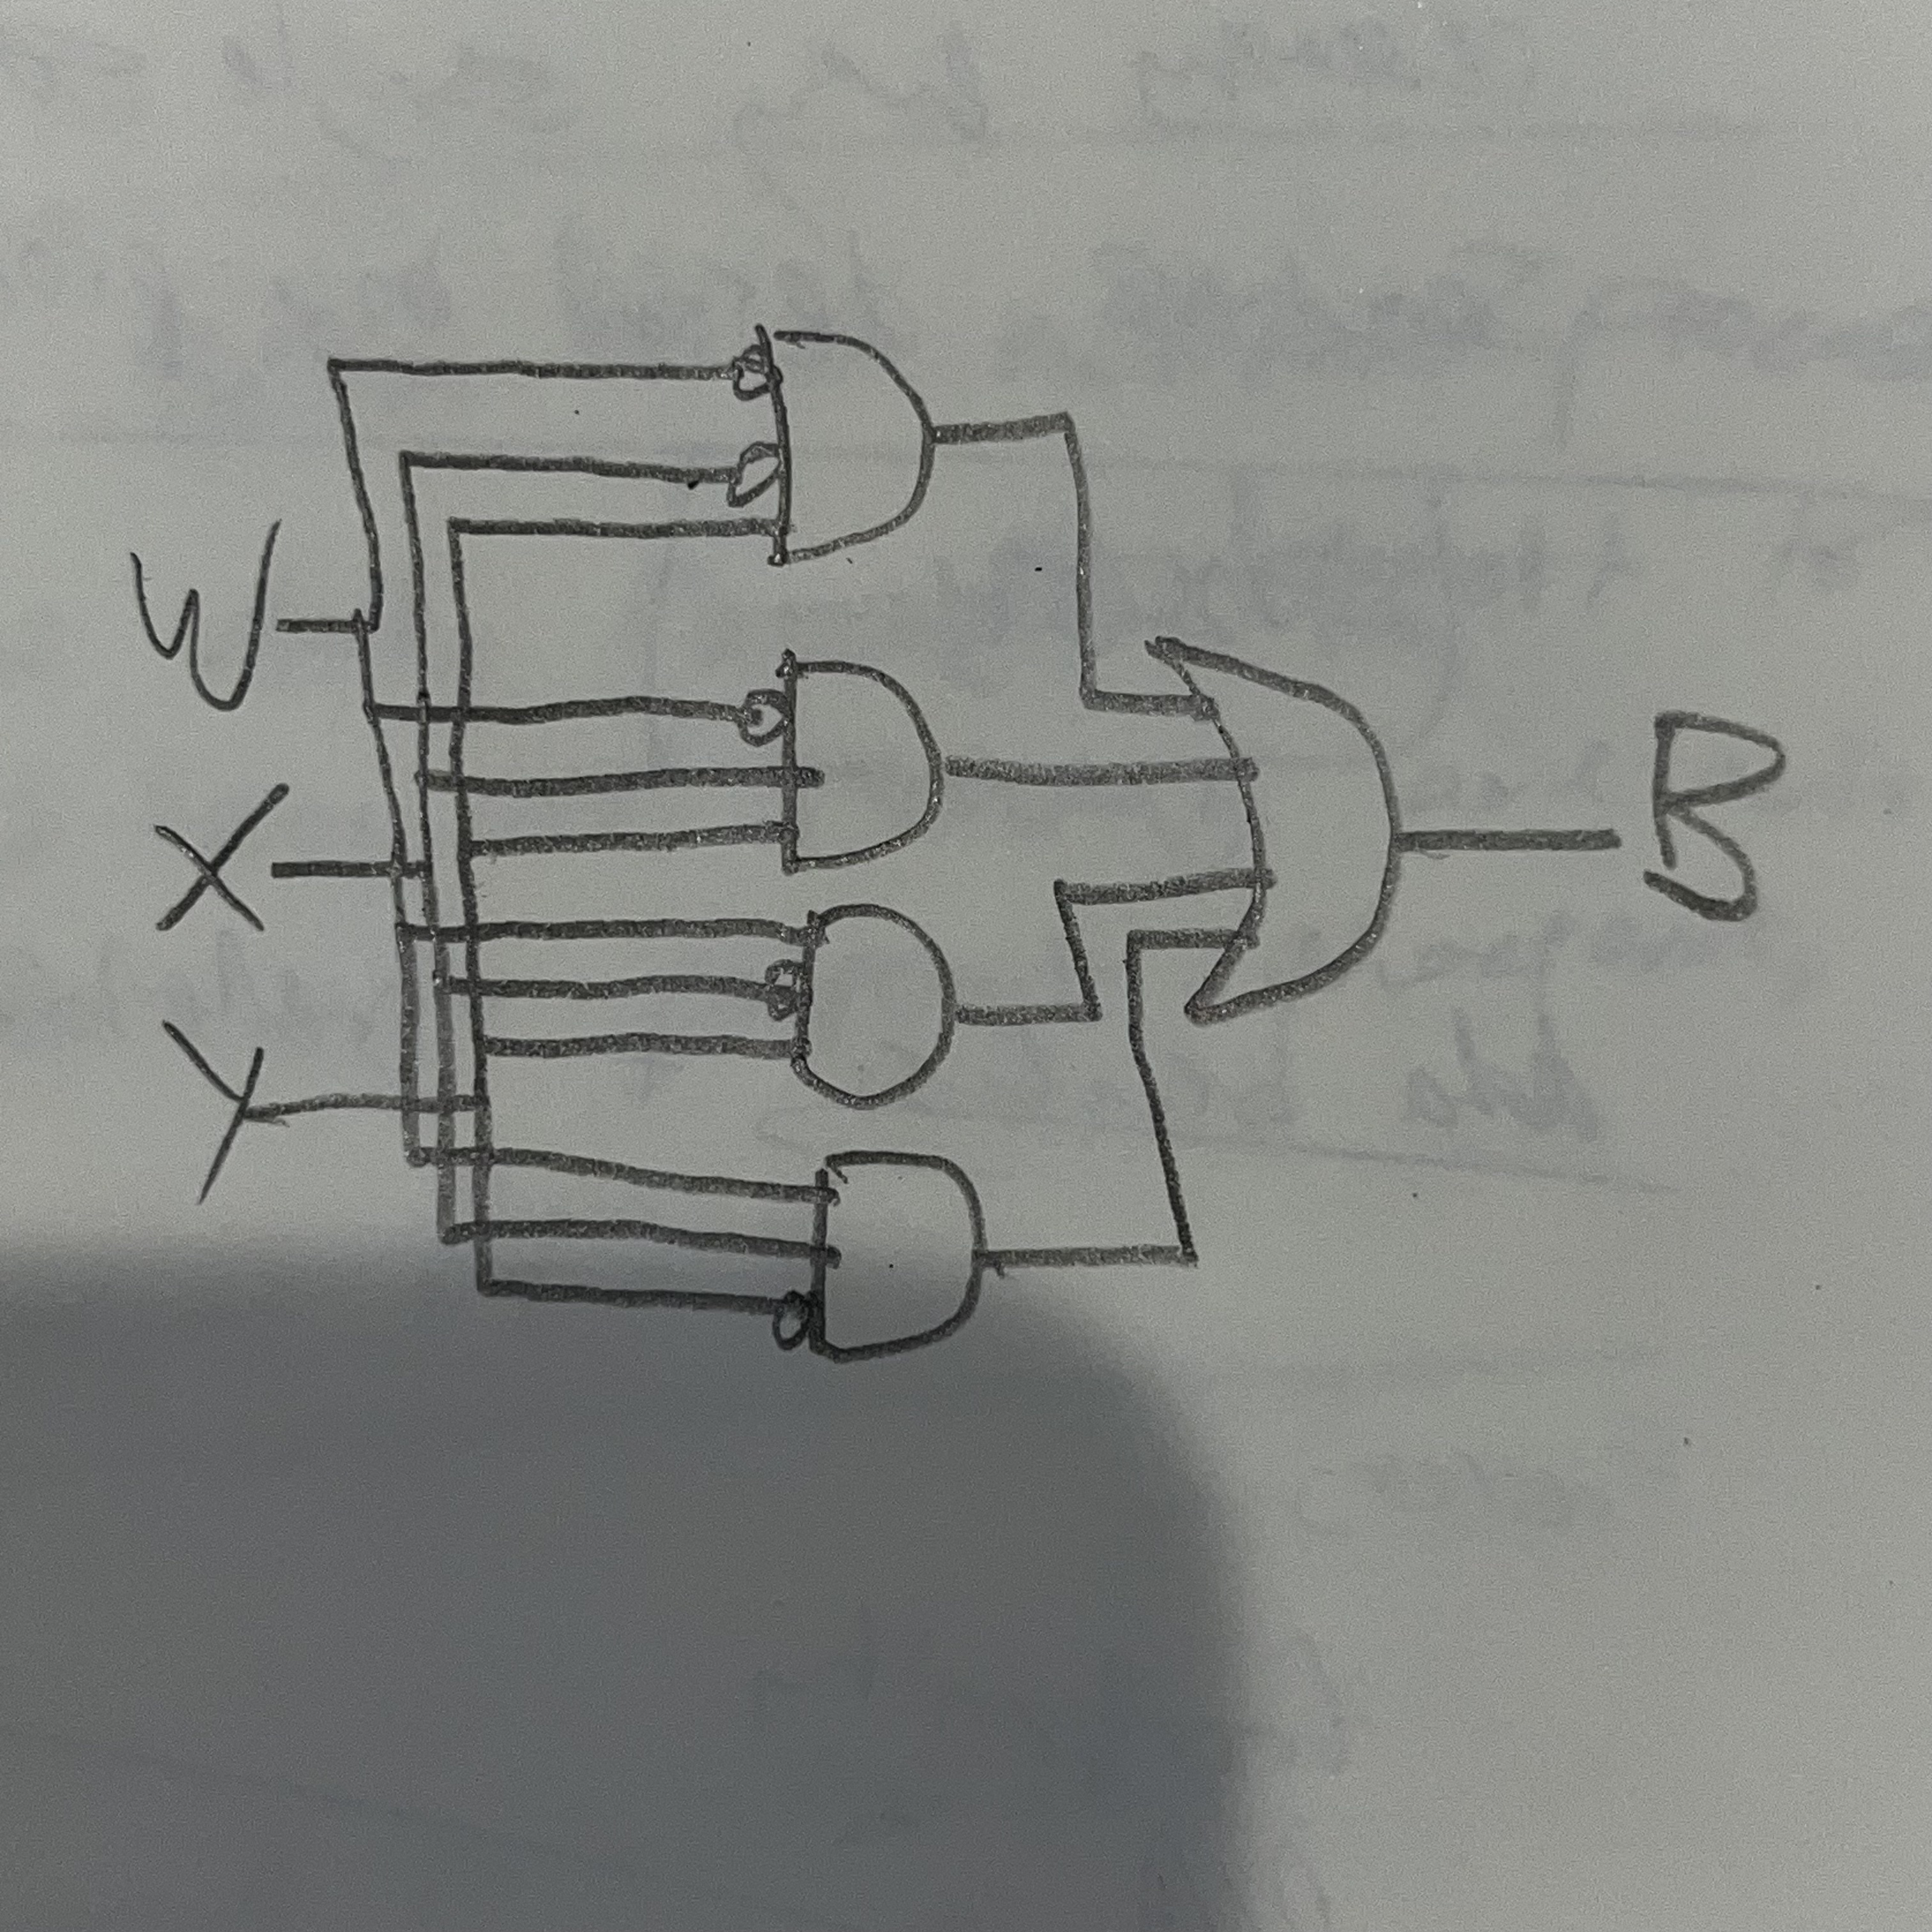
\includegraphics[width=0.3\textwidth]{./Images/B.jpeg}\\
        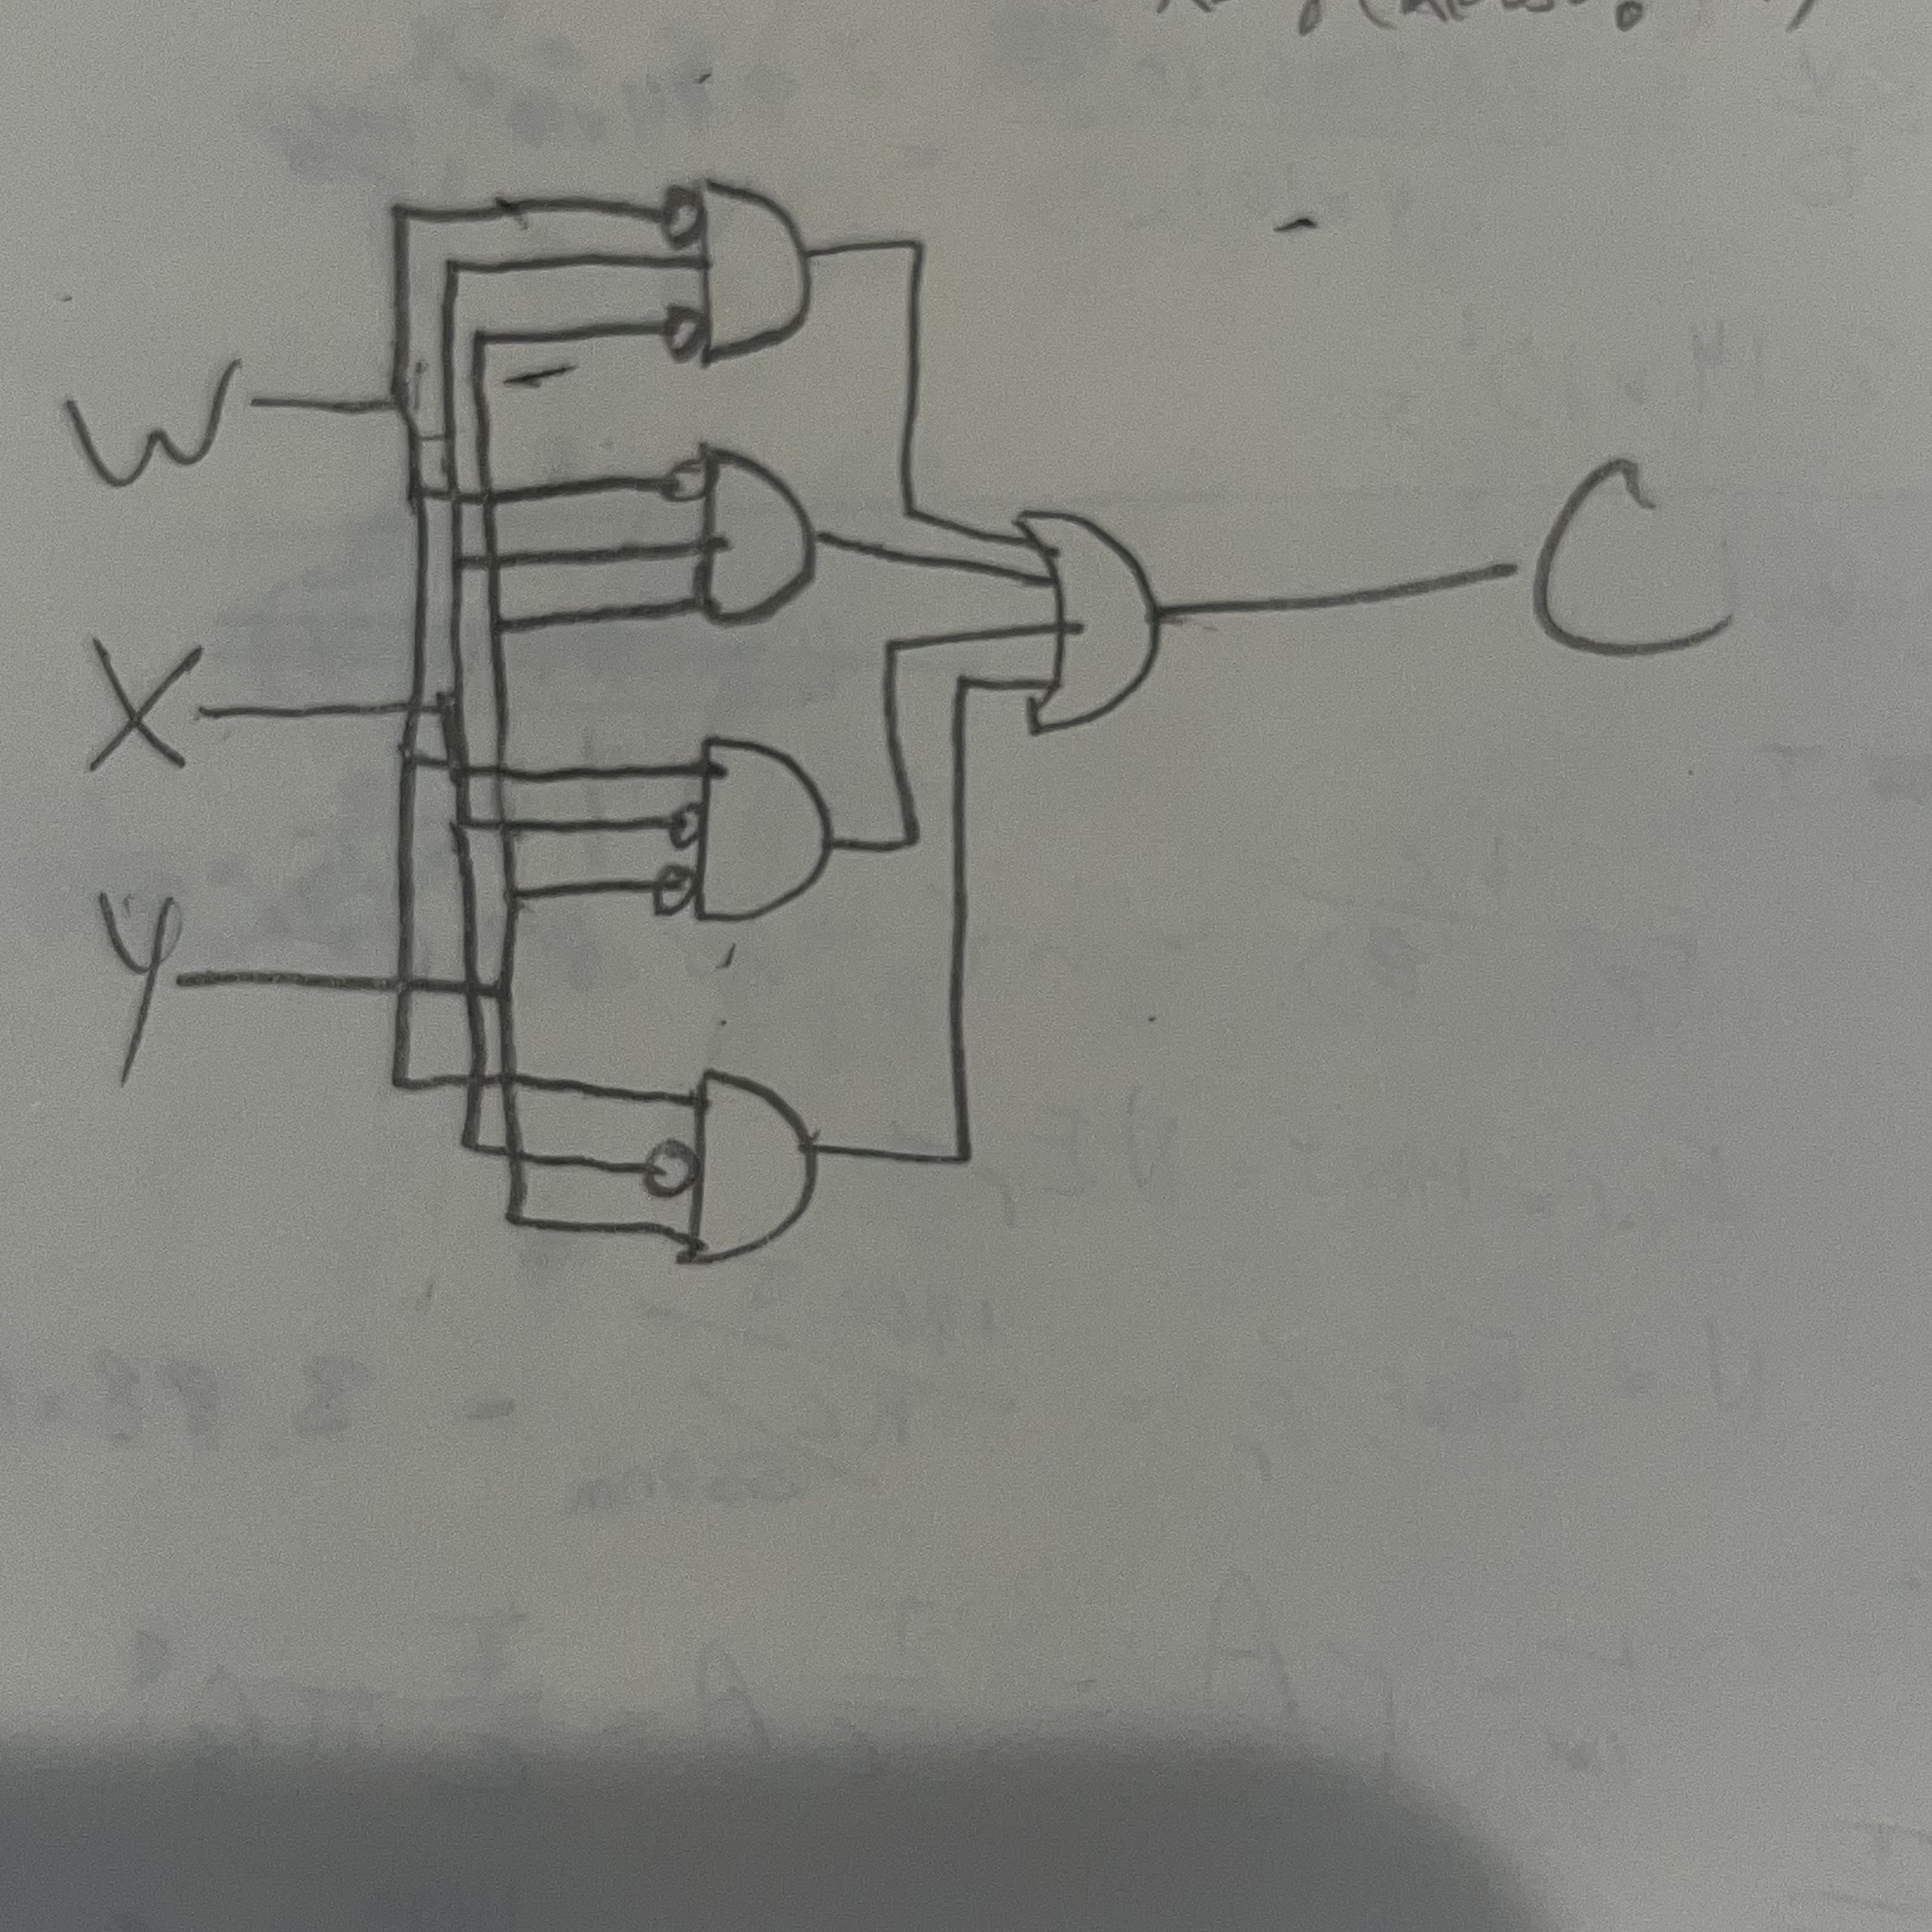
\includegraphics[width=0.3\textwidth]{./Images/C.jpeg}\\
      \end{tabular}
      \centering
      \caption{Unsimplified Logic Circuits}
      \end{figure}
    \item 
      \begin{align*}
        A&=W'X'Y'+W'X'Y+W'XY'+WX'Y'+WX'Y+WXY' \\
         &=(X'Y'+X'Y+XY')(W+W') \\
         &=X'(Y'+Y)+XY' \\
         &=X'+Y'
      \end{align*}
      \begin{align*}
        B&=W'X'Y+W'XY+WX'Y+WXY' \\
         &=Y(W'X'+W'X+WX')+WXY' \\
         &=Y(W'+X')+WXY'\\
         &=W'Y+X'Y+WXY'
      \end{align*}
      \begin{align*}
        C&=W'XY'+W'XY+WX'Y'+WX'Y \\
         &=W'(XY'+XY)+W(X'Y'+X'Y) \\
         &=W'X+WX'
      \end{align*}
    \item 
      \begin{equation*}
        C=W\oplus X
      \end{equation*}
  \end{enumerate}
\item . \\
    \begin{tabular}{|l|l|l|l||l|}
      \hline
      \textbf{A}	 & 	\textbf{B}	 & 	\textbf{C}	 & 	\textbf{D}	 & 	\textbf{X} \\ \hline
      0	 & 	0	 & 	0	 & 	0	 & 	1 \\ \hline
      0	 & 	0	 & 	0	 & 	1	 & 	1 \\ \hline
      0	 & 	0	 & 	1	 & 	0	 & 	1 \\ \hline
      0	 & 	0	 & 	1	 & 	1	 & 	1 \\ \hline
      0	 & 	1	 & 	0	 & 	0	 & 	0 \\ \hline
      0	 & 	1	 & 	0	 & 	1	 & 	1 \\ \hline
      0	 & 	1	 & 	1	 & 	0	 & 	0 \\ \hline
      0	 & 	1	 & 	1	 & 	1	 & 	0 \\ \hline
      1	 & 	0	 & 	0	 & 	0	 & 	0 \\ \hline
      1	 & 	0	 & 	0	 & 	1	 & 	1 \\ \hline
      1	 & 	0	 & 	1	 & 	0	 & 	1 \\ \hline
      1	 & 	0	 & 	1	 & 	1	 & 	1 \\ \hline
      1	 & 	1	 & 	0	 & 	0	 & 	0 \\ \hline
      1	 & 	1	 & 	0	 & 	1	 & 	1 \\ \hline
      1	 & 	1	 & 	1	 & 	0	 & 	0 \\ \hline
      1	 & 	1	 & 	1	 & 	1	 & 	0 \\ \hline
      \end{tabular}

\end{enumerate}

\end{document}

